\documentclass[12pt, c]{beamer}
% Setup appearance:

% Standard packages
\usepackage[francais]{babel}
\usepackage[latin1]{inputenc}
\usepackage{times}
\usepackage[T1]{fontenc}
\usepackage{float}
\usepackage{multirow}
\usepackage{subfigure}
\usepackage{pifont}
\usepackage{tikz}
\usepackage{morewrites}
%\usepackage{subfig}
\usetikzlibrary{arrows}
\tikzstyle{block}=[draw opacity=0.7,line width=1.4cm]
\DeclareOption{english}{\trans@use@and@alias{english}{English}}
\ProcessOptions*

\mode<presentation> {
	\definecolor{bgcol}{RGB}{255,255,255}
	\definecolor{grencol}{RGB}{0,102,0}
	\definecolor{rulecol}{RGB}{3,16,67}
	\definecolor{boxtitre}{RGB}{37,45,137}
	}

  \usetheme{Warsaw}
	%\usecolortheme[named=rulecol]{structure}
	\usefonttheme[onlysmall]{structurebold}
	\usefonttheme{structureitalicserif}
	\useinnertheme{rounded}
	\useoutertheme{split}
	
	\beamertemplateshadingbackground{bgcol}{bgcol} % pour jouer sur la couleur % du fond
	\beamertemplatetransparentcovereddynamic
	\setbeamertemplate{background canvas}[vertical shading][top=white, bottom=white!60!white]
	%\setbeamercolor{normal text}{bg=rulecol,fg=black}
	%\setbeamercolor{title in head}{bg=rulecol!80,fg=bgcol}
	\setbeamercolor{title in foot}{bg=black,fg=white}
	\setbeamercolor{author in head}{bg=rulecol,fg=bgcol}
	\setbeamercolor{author in foot}{bg=black!80,fg=white}
	\setbeamercolor{section in head}{bg=black,fg=bgcol}
	\setbeamercolor{section in foot}{bg=rulecol!80,fg= bgcol}
	\setbeamercolor{subsection in head}{bg=black,fg=bgcol}
	\setbeamercolor{subsection in foot}{bg=rulecol,fg=bgcol}
	\setbeamercolor{logo}{bg=rulecol,fg=white}
	\setbeamercolor{section in head/foot}{bg=black!90,fg=white}
	\setbeamercolor{subsection in head/foot}{bg=rulecol!90,fg=white}
	\setbeamercolor{boiterouge}{bg=red!60,fg=black}
	\setbeamercolor{boiterougeB}{bg=red,fg=black}
	\setbeamercolor{boiteblanche}{bg=white,fg=black}
	\setbeamercolor{boiteverte}{bg=green,fg=black}
	\setbeamercolor{boiteblue}{bg=rulecol,fg=white}
	
	\setbeamerfont*{frametitle}{size=\normalsize}
	
	
  \setbeamertemplate{navigation symbols}{}
	\setbeamertemplate{itemize item}[square]
	\setbeamertemplate{enumerate item}[ball]
	\setbeamertemplate{itemize subitem}[triangle]
	\setbeamertemplate{itemize subsubitem}[circle]
	\logo{
\includegraphics[height=5mm]{images/logouniv.png}}
	\setbeamertemplate{footline}{
		\leavevmode%
		\hbox{\hspace*{-0.06cm}
		
		\begin{beamercolorbox}[wd=.265\paperwidth,ht=2.25ex,dp=1ex,left]{author in foot}%
			\usebeamerfont{author in head/foot}\insertshortauthor%~~(\insertshortinstitute)
		\end{beamercolorbox}%
		
		\begin{beamercolorbox}[wd=.6\paperwidth,ht=2.25ex,dp=1ex,center]{title in foot}%
			\usebeamerfont{title in head/foot}\insertshorttitle
		\end{beamercolorbox}%
		
		\begin{beamercolorbox}[wd=.135\paperwidth,ht=2.25ex,dp=1ex,right]{section in foot}%
			\usebeamerfont{logo}\textcolor[rgb]{1,0.41,0.13}{\insertshortdate{}}\hspace*{0.4em}
			\insertframenumber{} / \inserttotalframenumber
		\end{beamercolorbox}}%
		
		\vskip0pt%
	}
\renewcommand{\raggedright}{\leftskip=0pt \rightskip=0pt plus 0cm}

\title[Secure Distributed Cluster Formation in Wireless Sensor Networks]{}

\author[$\;\;$ TCHIO AMOUGOU Styves Daudet]{}

\date[Janvier 2021]{janvier 2021}

%\subject{Mémoire de Master 2}
\begin{document}
\begin{frame}
\transfade
	\vspace{-0.3cm}
	\begin{figure}
		\begin{center}
		
\includegraphics[width=11cm,height=1.2cm]{images/enteteUds.PNG}
		\end{center}
	\end{figure}
	
	\begin{center}
	\tiny{\textsc{\textcolor{black}{DSCHANG SCHOOL OF SCIENCES AND TECHNOLOGY}}}\\
		\tiny{Unité de Recherche en Informatique Fondamentale, Ingénierie et  Application (URIFIA)}
	\end{center}
	\vspace{0.05cm}
\fcolorbox{boxtitre}{boxtitre}{\parbox{1\linewidth}{

\vspace{-0.3cm}
\begin{center}

\vspace{0.05cm}
 \textcolor{bgcol}{Secure Distributed Cluster Formation in Wireless Sensor Networks}

%\vspace{0.1cm}
\end{center}

\vspace{-0.1cm}
}}
\begin{center}
\fcolorbox{bgcol}{bgcol}{
\parbox{1\linewidth}{
\begin{center}
\vspace{-0.5cm}
\footnotesize Présenté par :\\ \textbf{\textcolor{boxtitre}{ TCHIO AMOUGOU Styves daudet}} \\
\scriptsize{\textit{Matricule : CM-UDS-14SCI0251}}\\
 \tiny{\textit{Licencié en Informatique Fondamentale}}\\
 \vspace{0.3cm}
				\scriptsize{\textit{Sous la direction de }}\\
				\scriptsize{\textbf{Dr BOMGNI ALAIN Bertand} }\\
								\tiny{(\textit{Chargé de Cours, Université de Dschang})}\\
				\end{center}
}}
\end{center}
\end{frame}

\begin{frame}{\scriptsize Sommaire}
\transwipe
\scriptsize
  \tableofcontents
\end{frame}

\section{Introduction}
	\subsection{Contexte}
	\setbeamercovered{invisible}
	\begin{frame}{Context}
	\transwipe
	
	\vspace{-0.25cm}
	\begin{block}
		\scriptsize Dans les réseaux de capteurs les attaques malicieuses sont un problème réel, plusieurs protocoles proposés ne résistent pas aux attaques malicieuses dans des environnements hostiles.
		
	 En effet,Un noeud malicieux peut opérer sur deux niveaux:
							\begin{itemize}
								\item Les données échangées entre les noeuds
								\item La topologie du réseau créée par le protocole
							\end{itemize}

	\end{block}
	\end{frame}
	
	\begin{frame}{Contexte}
		\transwipe
		\vspace{-0.25cm}
		\begin{block}{Exemple Déattaque Active:}
			\begin{itemize}
				\item Attaque de "jamming" \\ Vu la sensibilité du média sans fil au bruit, un noeud peut provoquer un déni de service en émettant des signaux é une certaine fréquence. Cette attaque peut être très dangereuse car elle peut être menée par une personne non authentifiée et étrangère au réseau.
				\begin{figure}
		\begin{center}
		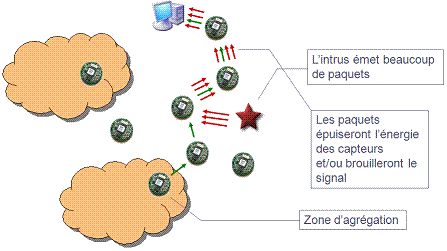
\includegraphics[width=10cm,height=4cm]{images/jamming.PNG}
		\end{center}
	\end{figure}
			\end{itemize}
		\end{block}
	\end{frame}
	
	\begin{frame}{Contexte}
		\transwipe
		\vspace{-0.25cm}
		\begin{block}{Exemple D'attaque Active:}
			\begin{itemize}
				\item ASink hole \\ Dans une attaque sinkhole, le noeud essaye d'attirer vers lui le plus de chemins possibles permettant le contrôle sur la plupart des données circulant dans le réseau. Pour ce faire, l'attaquant doit apparaître aux autres comme étant très attractif, en présentant des routes optimales.
				\begin{figure}
		\begin{center}
		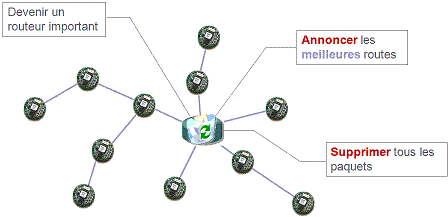
\includegraphics[width=10cm,height=4cm]{images/sinkhole.PNG}
		\end{center}
	\end{figure}
			\end{itemize}
		\end{block}
	\end{frame}
			

			
	\subsection{Problématique générale}		
			\begin{frame}{Problématique générale}
	\transglitter
				\begin{alertblock}{ Problématique générale}
					\large Détection des noeuds malicieux dans les réseaux de capteurs.
				\end{alertblock}
				\begin{figure}%
				\centering
				
\includegraphics[width=2cm, height=3cm]{images/bonhomme_question.JPG}%
				\end{figure}
			\end{frame}	
						
\section{ secure distributed cluster formation in wireless sensor networks}	
			\begin{frame}{}
				\transfade
				\begin{center}
					\vspace{-0.2cm}
				\huge\textbf{ \textsc{ secure distributed cluster formation in wireless sensor networks}}
				\end{center}
			\end{frame}
			\subsection{Propriétés}
			\begin{frame}{Propriétés}
				\transwipe
				\vspace{-0.21cm}
					\begin{block}{\scriptsize Le protocole de formation de cluster distribué sécurisé possède les propriétés suivantes même s'il y a des attaquants externes et internes}
						\begin{itemize}
							\item[\ding{43}]Le protocole est entièrement distribué. Chaque noeud calcule sa clique uniquement en utilisant les informations de ses voisins;
							\item[\ding{43}] La fin du protocole est garantie. Les noeuds participants qui ne respectent pas les spécifications du protocole (p. ex., envoyer des messages contradictoires) seront identifiés et retirés de toutes les cliques;
						\end{itemize}
					\end{block}
					
			\end{frame}
			\begin{frame}{Propriétés}
				\transwipe
				\vspace{-0.21cm}
					\begin{block}{\scriptsize Le protocole de formation de cluster distribué sécurisé possède les propriétés suivantes même s'il y a des attaquants externes et internes}
						\begin{itemize}
						\item[\ding{43}] Une fois le protocole terminé,
						\begin{itemize}
										\item Tous les noeuds normaux sont divisés en cliques disjointes.
										\item  Tous les noeuds normaux sont garantis d'avoir des vues cohérentes sur leurs adhésions é la clique, même dans un environnement hostile;

									\end{itemize}
						\end{itemize}
					\end{block}
					
			\end{frame}
			\begin{frame}{propriétés}
				\transwipe
					\vspace{-0.21cm}
						\begin{block}{\scriptsize Le protocole de formation de cluster distribué sécurisé possède les propriétés suivantes même s'il y a des attaquants externes et internes}
							\begin{itemize}
								\item[\ding{43}]les attaquants internes qui ne suivent pas la sémantique du protocole peuvent étre identifiés et retirés du réseau ;
								\item[\ding{43}] les attaquants externes peuvent être empêchés de participer au processus de formation du cluster;
								
								\item[\ding{43}]  les coûts de communication sont modéré
							\end{itemize}
						\end{block}
			\end{frame}
			\subsection{Hypothèses }
				\begin{frame}{Hypothèses }
					\transwipe
					\vspace{-0.21cm}
					\begin{block}{}
							\begin{itemize}
								\item[\ding{43}]Chaque 	\tiny{noeud} connaît ses voisins 1-hop
								\item[\ding{43}]Les noeuds de capteurs peuvent effectuer des opérations de signature numérique é clé publique.

								\item[\ding{43}]Les horloges des noeuds normaux sont synchronisées de manière lâche, comme l'exige uTESLA.
								\item[\ding{43}]Les clés publiques utilisées par les noeuds capteurs sont correctement authentifiées
 
							\end{itemize}
					
					\end{block}
				\end{frame}
			\subsection{Protocol Specification}
				\begin{frame}{Spécification du protocole}
					\transwipe
					\vspace{-0.21cm}
					\begin{block}{}
							\begin{itemize}
								\item[\ding{43}] étape 1: Chaque noeud échange ses listes de voisins avec ses voisins et calcule sa clique maximale locale.
								\item[\ding{43}]étape 2: Chaque noeud:
									\begin{itemize}
										\item échange sa clique maximale locale avec ses voisins,
										\item et met é jour sa clique maximale en fonction  cliques maximales locales de ses noeuds voisins.
									\end{itemize}
								\item[\ding{43}] étape 2: Chaque noeud: 
										\begin{itemize}
										\item échange la clique mise é jour avec ses voisins
										\item et calcule sa clique finale
									\end{itemize}
							\end{itemize}
					\end{block}
				\end{frame}
				\begin{frame}{Spécification du protocole}
					\transwipe
					\vspace{-0.21cm}
					\begin{block}{}
							\begin{itemize}
								\item[\ding{43}]étape 4: Chaque noeud échange le clic final avec ses voisins.
								
									\begin{itemize}
										\item Si aucune incohérence de clique n'est détectée, il se termine avec succès.
										\item
Sinon, il entre é l'étape 5.
									\end{itemize}
								
								 
								\item[\ding{43}]étape 5: Chaque noeud effectue un contrôle de conformité.
									\begin{itemize}
										\item 
S'il identifie les noeuds (voisins) malveillants, il les supprime du réseau et redémarre le protocole é partir de l'étape 1.
										\item Sinon, il applique l'accord de clique et prend fin.
									\end{itemize}									 

							\end{itemize}
					\end{block}
				\end{frame}
				\subsection{Limite}
					\begin{frame}{Limite}
						\transwipe
						\vspace{-0.21cm}
						\begin{block}{}
							\begin{itemize}
								\item[\ding{43}]Actuellement, le protocole est adapté aux réseaux de capteurs statiques, dans lesquels les noeuds ne se déplacent pas fréquemment
							\end{itemize}
						\end{block}
					\end{frame}
			
	
		
		\begin{frame}
\transdissolve
	\vspace{1cm}
	\begin{center}
	\huge \textbf{\textsc{Merci pour votre aimable attention}}
	\end{center}
\end{frame}
	
%\bibliographystyle{apacite} 
%\bibliography{References/references}

%\subject{Mémoire de Master 2}
\begin{frame}
\transfade
	\vspace{-0.3cm}
	\begin{figure}
		\begin{center}
		
\includegraphics[width=11cm,height=1.2cm]{images/enteteUds.PNG}
		\end{center}
	\end{figure}
	
	\begin{center}
	\tiny{\textsc{\textcolor{black}{DSCHANG SCHOOL OF SCIENCES AND TECHNOLOGY}}}\\
		\tiny{Unité de Recherche en Informatique Fondamentale, Ingénierie et  Application (URIFIA)}
	\end{center}
	\vspace{0.05cm}
\fcolorbox{boxtitre}{boxtitre}{\parbox{1\linewidth}{

\vspace{-0.3cm}
\begin{center}

\vspace{0.05cm}
 \textcolor{bgcol}{Secure Distributed Cluster Formation in Wireless Sensor Networks}

%\vspace{0.1cm}
\end{center}

\vspace{-0.1cm}
}}
\begin{center}
\fcolorbox{bgcol}{bgcol}{
\parbox{1\linewidth}{
\begin{center}
\vspace{-0.5cm}
\footnotesize Présenté par :\\ \textbf{\textcolor{boxtitre}{ TCHIO AMOUGOU Styves daudet}} \\
\scriptsize{\textit{Matricule : CM-UDS-14SCI0251}}\\
 \tiny{\textit{Licencié en Informatique Fondamentale}}\\
 \vspace{0.3cm}
				\scriptsize{\textit{Sous la direction de }}\\
				\scriptsize{\textbf{Dr BOMGNI ALAIN Bertand} }\\
								\tiny{(\textit{Chargé de Cours, Université de Dschang})}\\
				\end{center}
}}
\end{center}
\end{frame}
\end{document}